\section{Introduction}
Software-Defined Networking (SDN) is a promising advancement in networking, allowing users to continuously describe complex and flexible policies for forwarding traffic on their networks. Although it has mainly been considered in the Local Area Network (LAN) setting, there is a desire to see it applied to the Wide Area Network (WAN) setting as well. 
A natural way to introduce SDN to the wide area setting is by adding SDN support to Internet Exchange Points (IXPs). At an IXP, tens to hundreds of Autonomous Systems (ASes) come together at a single location to exchange routing information via BGP and interdomain traffic via layer 2 forwarding. Because of this relatively simple centralized structure, IXPs can provide a way to quickly add the power of SDN to significant portions of interdomain traffic. 

Unfortunately, it has proven difficult to add SDN capabilities to an IXP in a scalable way. There are many challenges that must be addressed, including how to compile together the policies of multiple participants, how to ensure BGP routing is not violated, and how to incrementally deploy such a system. One of the most challenging obstacles has been preventing the violation of BGP routing by participant policies, and it is this obstacle that we will focus on. 


\subsection{Software-Defined IXP}

\begin{figure}[t!] 
\begin{minipage}{1\linewidth}
\begin{subfigure}[b]{0.96\linewidth}
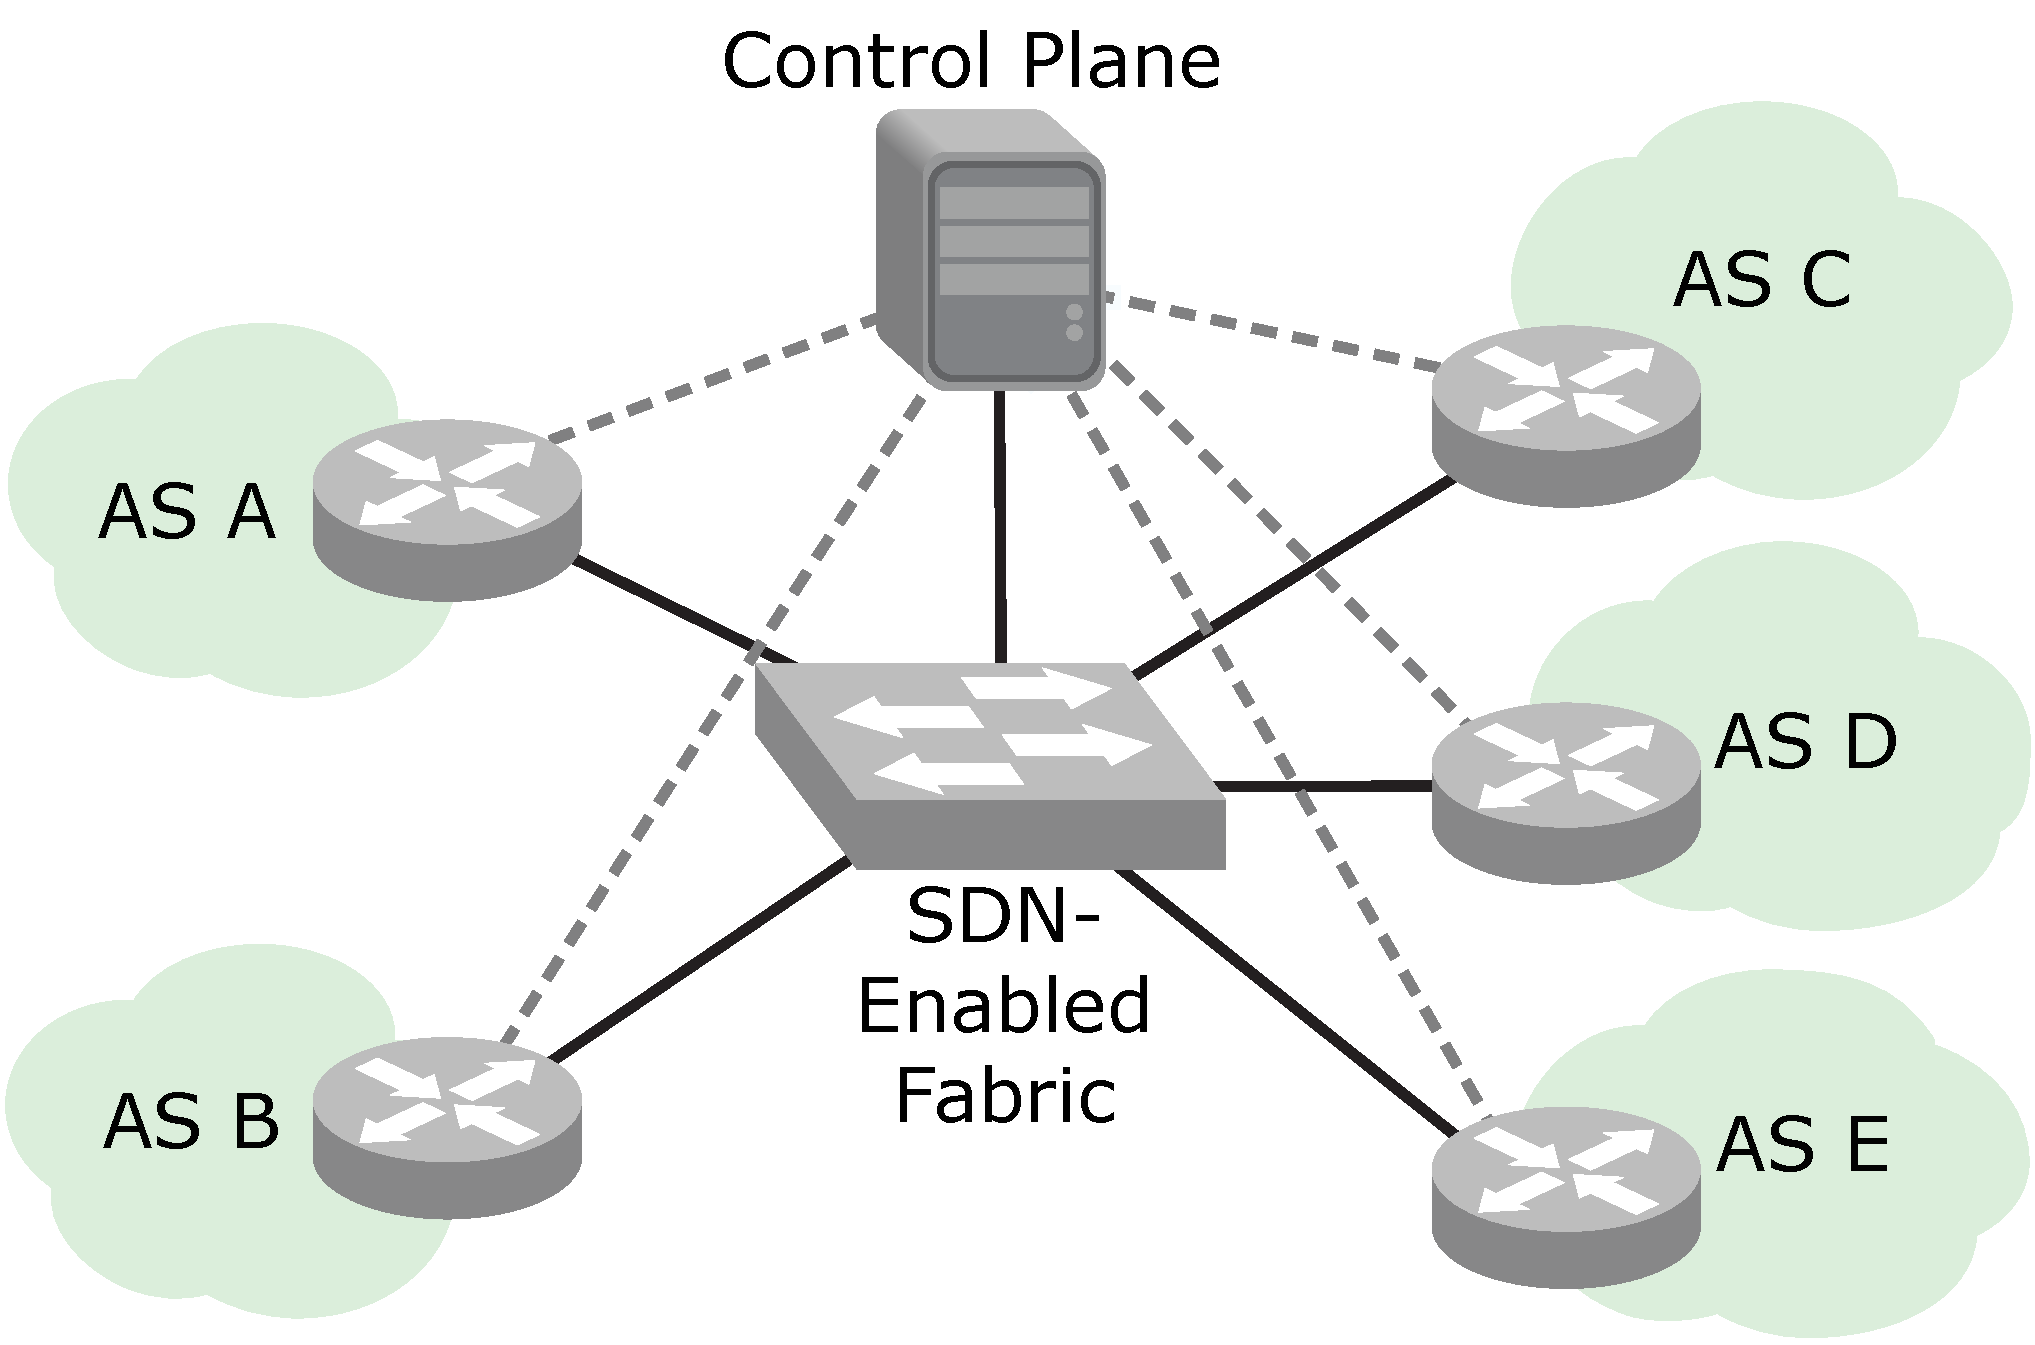
\includegraphics[width=\linewidth]{figures/sdx_example1}
\end{subfigure} 
\end{minipage} 
\caption{An example of a Software-Defined IXP. Pictured are 5 participant Autonomous Systems connected to the IXP's fabric and controller. Participants relay the policies they wish to install to the controller, which then installs it on their behalf on the fabric.}
\label{fig:sdx}
\end{figure}

Before we dive into the problem, we will give a brief description of an exchange point. An IXP consists a route server, traffic fabric, and participant AS border routers. An example is shown in figure \ref{fig:sdx}. Each border router connects to both the route server and the traffic fabric. Border routers send IP prefix route announcements and withdrawals to the route server via BGP messages, and the route server relays this information to the other participants' border routers. Each border router decides upon a \textit{default next-hop} for each prefix based upon the advertised routes it receives, and then sends traffic to those next-hops via the IXP fabric. 

In a Software-Defined IXP, the setup is similar but enhanced. There are still border routers connected to a fabric and a route server, but the route server now doubles as an SDN controller, connecting directly to the fabric to install forwarding table entries. The fabric now supports these SDN forwarding table entries, and can communicate with the controller via some SDN protocol such as OpenFlow~\cite{openflow}. Participants that wish to express SDN policies relay their policies to the controller, and the controller installs the policies into the fabric on their behalf. The controller determines how best to combine all the participants' policies to prevent conflict.

Participants can express two kinds of policies at a Software-Defined IXP: outbound policies and inbound policies. Outbound policies are forwarding actions applied to traffic which a participant sends \textit{to} the exchange point, and overrides the participants' default next-hop preferences when applied. Inbound policies are forwarding actions applied to traffic which a participant \textit{receives} from the exchange point, and is useful for dropping unwanted traffic or for when a participant has multiple connections to the exchange and wishes to apply some form of load balancing. 

Inbound policies are relatively straightforward to install at the exchange point, because all ports for a single participant lead to the same set of destinations and thus policies are not conditional upon available routes. Outbound policies, however, have proven difficult to correctly implement in the limited space of the forwarding plane. Throughout this work, we will be focusing on the compression of outbound policies and thus we will use the terms ``outbound policy" and ``policy" interchangeably. 
